\documentclass[a4paper]{article}

%% Language and font encodings
\usepackage[english]{babel}
\usepackage[utf8x]{inputenc}
\usepackage[T1]{fontenc}

%% Sets page size and margins
\usepackage[a4paper,top=3cm,bottom=2cm,left=3cm,right=3cm,marginparwidth=1.75cm]{geometry}

%% Useful packages
\usepackage{amsmath,amsthm,amssymb}
\usepackage{graphicx}
\usepackage[colorinlistoftodos]{todonotes}
\usepackage[colorlinks=true, allcolors=blue]{hyperref}
\newtheorem{theorem}{Theorem}
\newtheorem{lemma}{Lemma}
\newtheorem{remark}{Remark}
\newtheorem{example}{Example}
\newtheorem{corollary}{Corollary}




\newcommand{\dt}{\Delta t}
\newcommand{\dx}{\Delta x}
\newcommand{\te}{\theta}
\newcommand{\nul}{\nu_L(k,\theta)}
\newcommand{\nur}{\nu_R(k,\theta)}
\newcommand{\yl}{y_L(k,\theta)}
\newcommand{\yr}{y_R(k)}
\newcommand{\nplus}{\mathbb{N}^+}
\newcommand{\rr}{\mathbb{R}}
\newcommand{\Por}{P_{R,k}(y)}
\newcommand{\Pol}{P_{L,k,\te}(y)}
\newcommand{\cP}{{\cal{P}}}
\newcommand{\cD}{{\cal{D}}}






\title{Positivity of implicit discretizations of the advection equation}
\author{Yiannis Hadjimichael \and David I. Ketcheson \and Lajos L\'oczi}

\begin{document}
\maketitle

\section{Background and motivation}
Here we investigate the positivity of some discretizations of the advection equation
\begin{align} \label{advection}
U_t = a U_x.
\end{align}
The advection equation is a fundamental PDE, and herein we focus on
some of the simplest and most fundamental discretizations of it.

Any linear one-step discretization of a time-dependent PDE in one spatial
dimention with $m$ grid points in space yields an approximate solution given by
an iteration of the form
where $M$ is a fixed $m\times m$ matrix.


\subsection{Discrete Fourier analysis}
Any finite difference semi-discretization of \eqref{advection} with
periodic boundary conditions yields a system of ODEs
\begin{align} \label{semi-discrete}
    u'(t) & = \frac{a}{\dx}Lu(t)
\end{align}
where $L$ is a circulant matrix, which has the eigendecomposition
\begin{align}
    L & = F \Lambda F^*
\end{align}
where the (unitary) matrix of eigenvectors has entries
\begin{align}
    f_{jk} & = \exp(i \xi_k (j-1))/\sqrt{m}  & 1 \le j, k \le m
\end{align}
and $\Lambda$ is the diagonal matrix of eigenvalues, which depends on the
particular finite difference method chosen.  Here $\xi_k$ are the
$m$th roots of unity:
\begin{align}
    \xi_k & = \frac{2\pi(k-1)}{m} & 1 \le k \le m.
\end{align}

Applying a one-step time
discretization with stability function $R(z)$ to \eqref{semi-discrete} leads to
the iteration
\begin{align} \label{M}
    u^{n+1} & = R(\nu L) u^n = Mu^n
\end{align}
where $M=F^* R(\nu \Lambda) F$ and $\nu=a\dt/\dx$ is the CFL number.  The
necessary and sufficient condition for positive invariance of the numerical
solution is then simply that every entry of $M$ be nonnegative.

Note that $M$ is also a real, circulant matrix.
Thus it is defined completely by the entries of its first row, which
are given by
\begin{align} \label{M-entries}
    M_{1,j} & = \frac{1}{m} \sum_{k=1}^m R(\nu\lambda_k) \exp(-i(j-1)\xi_k).
\end{align}

\section{Backward in time, centered in space}
Consider the case of a 3-point centered difference in space:
\begin{align}
    U_x|_{x=x_j} \approx \frac{u_{j+1}-u_{j-1}}{2\dx}
\end{align}
so that $L$ is a circulant matrix with entries $(-1/2, 0, 1/2)$ on the central
three diagonals.  The exact solution of the resulting semi-discrete
system \eqref{semi-discrete} is not positive invariant, so (given an appropriate
positive initial condition) any consistent time discretization will yield
negative values for small enough time steps.  Here we investigate whether
it is possible to ensure positive invariance for large time steps.

Let us consider first the backward Euler method.
The eigenvalues for this semi-discretization are $\lambda_j = i\sin\xi_j$.
If we use the backward Euler method in time, we have $R(z) = (1-z)^{-1}$, so
\eqref{M-entries} gives the entries of $M$ as
\begin{align} \label{firstrow}
    M_{1,j} & = \frac{1}{m} \sum_{k=1}^m \frac{\exp\left(-i(j-1)\xi_k\right)}{1-\nu i \sin\xi_k}.
\end{align}
If $m$ is even, then these entries cannot all be positive.

\begin{lemma}
    If $m$ is even, then $M_{1,m} < 0$.
\end{lemma}
\begin{proof}
    From \eqref{firstrow} we have
    \begin{align}  \label{M12}
        M_{1,m} & = \frac{1}{m} \sum_{k=1}^m \frac{ \exp(-i(m-1)\xi_k)}{1-\nu i \sin\xi_k}
                  = \frac{1}{m} \sum_{k=1}^m \frac{ \exp(i\xi_k)}{1-\nu i \sin\xi_k}
                  = \frac{1}{m} \sum_{k=1}^m \frac{\cos \xi_k - \nu \sin^2 \xi_k}{1+\nu^2 \sin^2 \xi_k}.
    \end{align}
    The expression on the right is obtained by multiplying by the complex
    conjugate of the denominator and taking the real part (since $M$ is a real matrix).
    Due to symmetry, when $m$ is even,
    \begin{align*}
        \sum_{k=1}^m \frac{\cos \xi_k}{1+\nu^2\sin^2\xi_k}  = \sum_{k=1}^{m/2} \frac{\cos \xi_k + \cos(\xi_k+\pi)}{1+\nu^2\sin^2\xi_k} = 0.
    \end{align*}
    Thus 
    \begin{align*} 
        M_{1,m} & = \frac{1}{m} \sum_{k=1}^m \frac{- \nu \sin^2 \xi_k}{1+\nu^2 \sin^2 \xi_k} < 0.
    \end{align*}
\end{proof}
Using similar expressions, it can in fact be shown that, for $m$ even, we have
$M_{1,2j}<0$ for $1\le j \le m/4$; in other words, approximately one fourth of
the entries of $M$ are negative, no matter the value of $\nu$.  All of these
negative entries tend to zero as $\nu \to \infty$.

Meanwhile, if $m$ is odd...


In what follows we assume $m\ge 3$. Next we generalize the above results to the theta method.  In this case we have
\begin{align}
    R(z) & = \frac{1+(1-\theta)z}{1-\theta z}
\end{align}
so with the centered difference in space we get for $1\le j\le m$ that
\begin{align} \label{firstrow-theta}
    M_{1,j} & = \frac{1}{m} \sum_{\ell=1}^m \frac{1+\imath(1-\theta)\nu \sin(\xi_\ell)}{1-\imath\theta\nu \sin(\xi_\ell)}\exp\left(-\imath(j-1)\xi_\ell\right).
\end{align}
This leads to
\begin{align*} 
    M_{1,m} & = \frac{1}{m} \sum_{\ell=1}^m \frac{(1-\theta(1-\theta)\nu^2\sin^2(\xi_\ell))\cos(\xi_\ell)- \nu \sin^2 (\xi_\ell)}{1+\theta^2\nu^2 \sin^2 (\xi_\ell)}.
\end{align*}
For even $m=2k\ge 4$, the sum over the first term in the numerator vanishes due to symmetry and we have
\begin{align*}
    M_{1,2k} & =  \frac{1}{2k} \sum_{\ell=1}^{2k} \frac{- \nu \sin^2 (\xi_\ell)}{1+\theta^2\nu^2 \sin^2 (\xi_\ell)} < 0.
\end{align*}
\begin{remark}
By using \eqref{firstrow-theta} and similar symmetry arguments, one can prove that for any $m=2k\ge 4$ we have
\[
M_{1,2}=-M_{1,2k},
\]
from which one can also easily deduce that $M\ge 0$ is impossible for $\nu>0$ and $\te\in[0,1]$.
\end{remark}

\begin{theorem}
Consider the backward in time, centered in space discretization of the
advection equation with periodic boundary conditions and $m$ spatial grid
points.  The discretization takes the form \eqref{M},
where (i) if $m$ is even, then $M$ has at least one negative entry;
(ii) if $m$ is odd, then for $\dt>\dt_*$ all entries of $M$ are nonnegative.

(add details about $\dt_*$)
\end{theorem}

\subsection{Discrete Fourier analysis}
David's work here.

\subsection{Some material for: Notation/Introduction}

 Mention: enough to focus on the 1st row: the sum/product/inverse of circulant matrices is circulant [REFERENCE: Fact 5.16.7. in Berstein MATRIX MATHEMATICS]. Since $L$ and $I$ are circulant, the matrix $M$ is circulant, too.\\
Financial support for LL: TKP project + KAUST\\
We used Wolfram \textit{Mathematica} (version 11) for the computations in this work.




 We need the explicit form of $L$---the first row.\\

$M\ge 0$ means that  $M_{i,j}\ge 0$ for every entry $1\le i, j\le m$.\\

$M\not\ge 0$ means there is at least one negative entry $M_{i,j}<0$.\\

$\imath^2=-1$ 

$3\le m\in\nplus$

\begin{equation}\label{Mdef}
M(m,\te,\nu):=(I-\te\nu L)^{-1}(I+(1-\te)\nu L),
\end{equation}
where $I\in\rr^{m\times m}$ is the identity matrix. The dependence of $M$ on its parameters will often be suppressed. To emphasize the dimensions of a matrix, we will sometimes write, for example, $L_{m\times m}$.

\subsection{Explicit description of the matrix entries for odd values of $m$}\label{explsect}

When $m\ge 3$ is odd, it is not apparent how to use the trigonometric representation \eqref{firstrow-theta} to reveal information on the signs of the matrix entries $M_{1,j}$. Therefore, in this section, we first rewrite the  entries in a certain algebraic form by invoking some low-order linear recursions. Then, in Section \ref{nonnegsect}, we will give conditions for $M_{1,j}\ge 0$ in terms of the parameters $\te$ and $\nu$.
\begin{remark}
The results obtained in this section are independent of the question of non-negativity, and may be applicable in other contexts as well. 
\end{remark}




It is trivial that for $\te=0$ we have $M(m,0,\nu)=I+\nu L$, hence $M\ge 0$ cannot hold for any $\nu>0$. Thus, throughout the rest of this section, we can thus assume that 
\begin{equation}\label{genassump}
\boxed{ 
m=2k+1\quad (k\in\nplus), \ \ \ \nu>0 \text{\ \  and\ \  } 0<\te\le 1.}
\end{equation}
As an initial illustration, we present the first row of $M$ (as a vector, and with the common denominator of the entries in front of it) for the smallest values of $m$. 
\begin{example}\label{example1} 
%For $m=2$, 
%\[\frac{1}{{\theta ^2 \nu ^2}/{4}+1}\left(-\frac{1}{4} \theta ^2 \nu ^2+\frac{\theta  \nu ^2}{4}+1,\theta  \nu -\frac{\nu }{2}\right),\]
For $m=3$ the first row of \eqref{Mdef} is 
\[
\frac{1}{{3 \theta ^2 \nu ^2}/{4}+1}\left(\frac{3 \theta ^2 \nu ^2}{4}-\frac{\theta  \nu ^2}{2}+1,\frac{\theta  \nu ^2}{4}+\frac{\nu }{2},\frac{\theta  \nu ^2}{4}-\frac{\nu }{2}\right),
\]
while for $m=5$ we have 
\[
\frac{1}{{5 \theta ^4 \nu ^4}/{16}+{5 \theta ^2 \nu ^2}/{4}+1}\left(\frac{5 \theta ^4 \nu ^4}{16}-\frac{\theta ^3 \nu ^4}{4}+\frac{5 \theta ^2 \nu ^2}{4}-\frac{\theta  \nu ^2}{2}+1,\right.
\]
\[
\left.\frac{\theta ^3 \nu
   ^4}{16}+\frac{\theta ^2 \nu ^3}{4}+\frac{\nu }{2},\frac{\theta ^3 \nu ^4}{16}-\frac{\theta ^2 \nu ^3}{8}+\frac{\theta  \nu ^2}{4},\frac{\theta ^3
   \nu ^4}{16}+\frac{\theta ^2 \nu ^3}{8}+\frac{\theta  \nu ^2}{4},\frac{\theta ^3 \nu ^4}{16}-\frac{\theta ^2 \nu ^3}{4}-\frac{\nu }{2}\right).
\]

\end{example}


Each element of $M$ is a rational function in the variables $\te$ and $\nu$. From \eqref{Mdef} it is clear that 
\begin{equation}\label{M1jPjkDk}
M_{1,j}=\frac{\cP_{j,k}(\te,\nu) }{\cD_k(\te,\nu)}\quad\quad(j=1,2,\ldots,2k+1),
\end{equation}
where $\cP_{j,k}$ and $\cD_{k}$ are certain bivariate polynomials in $\te$ and $\nu$, and 
\begin{equation}\label{dendet}
\cD_k:=\det\left(I_{(2k+1)\times(2k+1)}-\te\nu L_{(2k+1)\times(2k+1)}\right).
\end{equation}
\begin{remark}
The subscripts of $\cP_{j,k}$ thus refer to the position of the polynomial within the first row of $M$, and the size of $M\in\mathbb{R}^{(2k+1)\times(2k+1)}$, respectively.
\end{remark}


The key to describing $M$ algebraically is the observation that the polynomials $\cP_{j,k}$ and $\cD_{k}$ satisfy certain low-order linear recursions with constant coefficients. Interestingly, the leftmost entry ($j=1$) behaves differently than the rest ($2\le j\le 2k+1$).


\begin{remark}
 \textit{Mathematica}'s  {\tt{FindLinearRecurrence}} command proved to be an efficient tool for discovering these linear recursions. 
\end{remark}
First, let us introduce some new variables. On the one hand, as suggested by Example \ref{example1}, it seems convenient to set
\[
\mu:=\te^2\nu^2>0.
\]
Then, due to the sign assumptions, $\sqrt{\mu}=\te\nu$. On the other hand, as we will soon see, the polynomial 
\[
\kappa ^2-\kappa  \left(1+\frac{\mu }{2}\right)+\frac{\mu ^2}{16}
\]
will appear as a (factor of a) characteristic polynomial, and its roots are
\begin{equation}\label{kappa12}
\kappa_{1,2}=\frac{2+\mu \pm 2 \sqrt{\mu +1}}{4}=\left(\frac{\sqrt{1+\mu}\pm 1}{2}\right)^2.
\end{equation}
This motivates us to introduce yet another variable, which will further simplify our exposition. We set
\begin{equation}\label{ydef01}
y:=\frac{\sqrt{1+\mu}-1}{\sqrt{\mu}}=\frac{\sqrt{1+\te^2\nu^2}-1}{\te\nu}\in (0,1).
\end{equation}
It is seen that the transformation
\[
(0,+\infty)\ni\mu \longleftrightarrow y\in(0,1)
\]
is a bijection. Moreover, the following (inverse) relations 
\[
\mu=\left(\frac{2y}{1-y^2}\right)^2,
\]
\[\mu y^2=2+\mu-2\sqrt{1+\mu},\]
\[\mu/y^2=2+\mu+2\sqrt{1+\mu},\]
and
\begin{equation}\label{fromytonu}
\nu=\frac{2y}{1-y^2}\cdot\frac{1}{\te}
\end{equation}
are easily verified. We can now start describing the entries of the first row of $M$.
\begin{remark}
Although the expressions $\cP_{j,k}$ and $\cD_{k}$ will become in general rational functions in the variable $y$, we still call them polynomials (referring to their structure in the original variables $\te$ and $\nu$). 
\end{remark}
$\bullet$ The polynomials $\cD_k$. By carrying out some determinant expansions, we see that the determinants \eqref{dendet} obey the second-order parametric recursion
\begin{equation}\label{Dkrec}
\cD_{k+2}=\left(1+\frac{\mu}{2}\right)\cD_{k+1}-\frac{\mu^2}{16}\cD_k
\end{equation}
with initial conditions
\[
\cD_1=1+\frac{3\mu}{4}, \quad \cD_2=1+\frac{5\mu}{4}+\frac{5\mu^2}{16}
\]
(cf.~Example \ref{example1}). After solving this recursion, we obtain
\[
\cD_k=\left(\frac{\sqrt{1+\mu}+1}{2}\right)^{2 k+1}- \left(\frac{\sqrt{1+\mu}-1}{2}\right)^{2 k+1},
\]
which, in terms of the variable $y$, becomes
\begin{equation}\label{expldet}
\cD_k=\frac{1-y^{4 k+2}}{\left(1-y^2\right)^{2 k+1} }.
\end{equation}

$\bullet$  The polynomials $\cP_{1,k}$. They satisfy the recursion 
\[
\cP_{1,k+2}=\left(1+\frac{\mu}{2}\right)\cP_{1,k+1}-\frac{\mu^2}{16}\cP_{1,k},
\]
that is, with coefficients being the same as in \eqref{Dkrec}, but with initial conditions
\[
\cP_{1,1}=1+\frac{3 \mu }{4}-\frac{\mu /\theta}{2  }, \quad \cP_{1,2}=1+\frac{5 \mu }{4}+\frac{5 \mu ^2}{16}-\frac{\mu/\theta }{2  }-\frac{\mu ^2/\theta}{4  }
\]
(cf.~Example \ref{example1}). By solving this recursion we derive that
\begin{equation}\label{P1kexpl}
\cP_{1,k}=\frac{\Pol}{  \left(1+y^2\right)\left(1-y^2\right)^{2 k+1}\theta},
\end{equation}
where the numerator is 
\begin{equation}\label{poldef}
\Pol:=-\theta  y^{4 k+4}-(\theta -2) y^{4 k+2}+(\theta -2) y^2+\theta.
\end{equation}
\begin{remark}
Here, the subscript $L$ stands for \emph{leftmost}. This polynomial will play a special role in the next section.
\end{remark}


$\bullet$  The polynomials $\cP_{2,k}$. They satisfy a third-order recursion in the variable $k$,
\begin{equation}\label{cP2rec}
\cP_{2,k+3}=\left(1+\frac{3\mu}{4}\right)\cP_{2,k+2}-\left(\frac{\mu }{4}+\frac{3 \mu ^2}{16}\right)\cP_{2,k+1}+\frac{\mu ^3}{64}\cP_{2,k},
\end{equation}
with initial conditions 
\[
\cP_{2,1}=\left(\frac{1}{2}+\frac{\sqrt{\mu }}{4}\right) \nu, \quad \cP_{2,2}=\left(\frac{1}{2}+\frac{\mu }{4}+\frac{\mu ^{3/2}}{16}\right) \nu,
\]
\[
\cP_{2,3}=\left(\frac{1}{2}+\frac{\mu }{2}+\frac{3 \mu ^2}{32}+\frac{\mu ^{5/2}}{64}\right) \nu.
\]
The  characteristic polynomial of recursion \eqref{cP2rec} is 
\[
\kappa ^3-\kappa ^2 \left(1+\frac{3 \mu }{4}\right)+\kappa  \left(\frac{\mu }{4}+\frac{3 \mu ^2}{16}\right)-\frac{\mu ^3}{64}=\left(\kappa-\frac{\mu }{4}\right)\left(\kappa ^2-\kappa  \left(1+\frac{\mu }{2}\right)+\frac{\mu ^2}{16}\right),
\]
hence the characteristic roots are $\kappa_{1,2}$ as in \eqref{kappa12}, and $\kappa_3={\mu }/{4}$. Based on this, one easily obtains the explicit solution as
\begin{equation}\label{cP2kexpl}
\cP_{2,k}=\frac{\nu  \left(1-y^2\right)^{1-2 k} \left(1+y^{2 k-1}+y^{2 k+1}-y^{4 k}\right)}{2 \left(1+y^2\right)}.
\end{equation}


$\bullet$  The polynomials $\cP_{3,k}$. They satisfy the same third-order recursion in the variable $k$ as \eqref{cP2rec},
\[
\cP_{3,k+3}=\left(1+\frac{3\mu}{4}\right)\cP_{3,k+2}-\left(\frac{\mu }{4}+\frac{3 \mu ^2}{16}\right)\cP_{3,k+1}+\frac{\mu ^3}{64}\cP_{3,k},
\]
but with initial conditions 
\[
\cP_{3,1}=\left(-\frac{1}{2}+\frac{\sqrt{\mu }}{4}\right) \nu, \quad \cP_{3,2}=\left(\frac{\sqrt{\mu} }{4}-\frac{\mu}{8}+\frac{\mu ^{3/2}}{16}\right) \nu,
\]
\[
\cP_{3,3}=\left(\frac{\sqrt{\mu }}{4}-\frac{\mu ^2}{32}+\frac{3 \mu ^{3/2}}{16}+\frac{\mu ^{5/2}}{64}\right) \nu.
\]
The explicit solution of this recursion is
\begin{equation}\label{cP3kexpl}
\cP_{3,k}=\frac{\nu  \left(1-y^2\right)^{1-2 k} \left(y-y^{2 k-2}+y^{2 k+2}+y^{4 k-1}\right)}{2 \left(1+y^2\right)}.
\end{equation}
\begin{remark}
We note that, for any \emph{fixed} $j\ge 2$, the polynomials $\cP_{j,k}$ satisfy the same third-order recursion \eqref{cP2rec} in the variable $k$, with triplets of initial conditions depending on $j$. However, we cannot use this approach to proceed, since setting up the initial conditions would require, among others, the knowledge of the  polynomials $\cP_{j,1}$ (for $j=2, 3$),  $\cP_{j,2}$ (for $j=4, 5$), $\cP_{j,3}$ (for $j=6, 7$), and so on. 
\end{remark}



$\bullet$  The polynomials $\cP_{j,k}$ ($4\le j\le 2k+1$, $k\ge 2$). They satisfy the following second-order recursion in the variable $j$ when $k$ is \emph{fixed} (hence having only finitely many terms for a particular $k$):  
\[
\cP_{j+2,k}=-\frac{2}{\sqrt{\mu }}\cP_{j+1,k}+\cP_{j,k}.
\]
For the initial conditions of this final recursion, we use the general forms of $\cP_{2,k}$ and $\cP_{3,k}$ in \eqref{cP2kexpl} and \eqref{cP3kexpl} to get for any $k\ge 1$ and $2\le j\le 2k+1$ that 
\begin{equation}\label{Pjkexpl}
\cP_{j,k}=\frac{\nu  \left(1-y^2\right)^{1-2 k}}{2 \left(1+y^2\right)}P_{j,k}(y), 
\end{equation}
where the polynomials $P_{j,k}$ are defined as
\begin{equation}\label{Pjky}
P_{j,k}(y):=(-1)^{j-1} y^{4 k+2-j}+y^{2 k-1+j}+(-1)^j y^{2 k+1-j}+y^{j-2}.
\end{equation}
As a special case, we set
\[
\Por:=P_{2k+1,k}(y),
\]
in other words we have
\begin{equation}\label{pordef}
\Por=y^{4 k}+y^{2 k+1}+y^{2 k-1}-1,
\end{equation}
where the subscript $R$ stands for \textit{rightmost}.


\begin{remark}
As a by-product, we have obtained the following set of identities by comparing the trigonometric and algebraic representations presented so far. They are also interesting from a structural point of view: although the number of terms in the trigonometric sums increases as $k$ gets larger, the polynomials in $y$ are sparse polynomials (also known as lacunary polynomials or fewnomials)---the number of terms does not increase as the polynomial degree increases.
\end{remark}
\begin{corollary}
With $M$ defined in \eqref{Mdef}, $\te>0$, $\nu>0$, $k\in\nplus$, $y=\frac{\sqrt{1+\te^2\nu^2}-1}{\te\nu}$, and $\xi_\ell  = \frac{2\pi(\ell-1)}{2k+1}$, we have that
\[
 \frac{1}{2k+1} \sum_{\ell=1}^{2k+1} \frac{1+\imath(1-\theta)\nu \sin(\xi_\ell)}{1-\imath\theta\nu  \sin(\xi_\ell)}=
\]
\[
M_{1,1}=\frac{\cP_{1,k}}{\cD_k}=
\]
\[
\frac{-\theta  y^{4 k+4}-(\theta -2) y^{4 k+2}+(\theta -2) y^2+\theta}{  \left(1+y^2\right)\left(1-y^{4 k+2}\right)\theta}.
\]
Moreover, for $j=2, 3, \ldots, 2k+1$ we have that
\[
\frac{1}{2k+1} \sum_{\ell=1}^{2k+1} \frac{1+\imath(1-\theta)\nu \sin(\xi_\ell)}{1-\imath\theta\nu \sin(\xi_\ell)}\exp\left(-\imath(j-1)\xi_\ell\right)=
\]
\[
M_{1,j}=\frac{\cP_{j,k}}{\cD_k}=
\]
\[
\frac{\nu  \left(1-y^2\right)^2 }{2 \left(1+y^2\right) \left(1-y^{4 k+2}\right)}\Big((-1)^{j-1} y^{4 k+2-j}+y^{2 k-1+j}+(-1)^j y^{2 k+1-j}+y^{j-2}\Big).
\]
In particular,
\[
\prod_{\ell=1}^{2k+1} (1-\imath\theta\nu \sin(\xi_\ell))=\cD_k=
\]
\[
\left(\frac{\sqrt{1+\te^2\nu^2}+1}{2}\right)^{2 k+1}- \left(\frac{\sqrt{1+\te^2\nu^2}-1}{2}\right)^{2 k+1}=
\frac{1-y^{4 k+2}}{\left(1-y^2\right)^{2 k+1} }.
\]


\end{corollary}

\subsection{Non-negativity of the matrix entries for odd values of $m$}\label{nonnegsect}

In this section we present a detailed description of the non-negativity properties of the matrix $M$, thanks to the explicit forms for the entries $M_{1,j}$ obtained in Section \ref{explsect}.

\begin{center}\boxed{\text{Throughout this section we again assume \eqref{genassump}.}}\end{center}

By taking into account \eqref{M1jPjkDk}, \eqref{expldet}, \eqref{P1kexpl}, \eqref{poldef}, \eqref{Pjkexpl}, \eqref{Pjky}, and the fact that now $y\in(0,1)$ (see \eqref{ydef01}), the following corollary is evident.
\begin{corollary}\label{cor2} For a given pair $(\te,\nu)$
\[
M_{1,1}(2k+1,\te,\nu)\ge 0 \quad \Longleftrightarrow \quad \Pol\ge 0\quad\text{ (see } \eqref{poldef}\text{)},
\]
and for any $2\le j\le 2k+1$
\[
M_{1,j}(2k+1,\te,\nu)\ge 0 \quad \Longleftrightarrow \quad P_{j,k}(y)\ge 0\quad\text{ (see } \eqref{Pjky}\text{)}.
\]
\end{corollary}
\begin{figure}
\begin{center}
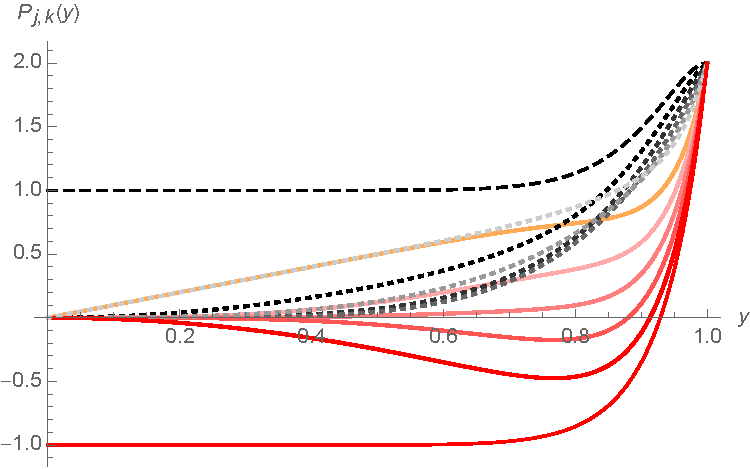
\includegraphics[width=0.5\textwidth]{fig_excepttopleft.pdf}
\caption{The typical behavior of the polynomials $P_{j,k}$ appearing in Corollary \ref{cor2} for $2\le j\le 2k+1$ and $k$ fixed: curves in shades of gray (or black) correspond to even $j$, while curves in shades of red (or orange) correspond to odd $j$ indices. Based on this figure, one can make the following observations. On the one hand, for each fixed and even $j$, $P_{j,k}$ is strictly increasing in $y$; however, for any fixed $y\in(0,1)$, $P_{j,k}$ is in general not monotone in its even index $j$. On the other hand, for each fixed and odd $j$, $P_{j,k}$ is in general not monotone in $y$; however, for any fixed $y\in(0,1)$, $P_{j,k}$ is strictly decreasing in its odd index $j$.}\label{fig_excepttopleft}
\end{center}
\end{figure}
The following lemma proves some of the observations about the polynomials $P_{j,k}$ suggested by Figure \ref{fig_excepttopleft} for even and odd indices $2\le j\le 2k+1$.
\begin{lemma}\label{lem2} Let us fix $y\in(0,1)$ arbitrarily. Then\\
\indent $\bullet$ for any $1\le\ell\le k$, $P_{2\ell,k}(y)>0$;\\
\indent $\bullet$ for any $2\le\ell\le k$, $P_{2\ell+1,k}(y)<P_{2\ell-1,k}(y)$. 
\end{lemma}
\begin{proof} For the even indices, we have
\[
P_{2\ell,k}(y)=y^{2 k-2 l+1}(1-y^{2 k+1})+y^{2 k+2 l-1}+y^{2 l-2}>0,\]
while for the odd indices,
\[
P_{2\ell+1,k}(y)-P_{2\ell-1,k}(y)=-(1 - y^2)\Big(y^{2 k+2 l-2}+y^{2 l-3}+y^{2 k-2 l}(1-y^{2k+1})\Big)<0.
\] 
\end{proof}
By combining Corollary \ref{cor2} and Lemma \ref{lem2}, we have obtained the following result, expressing the fact that the non-negativity of $M(2k+1,\te,\nu)$ is determined only by the polynomials appearing in the numerators of its top left and top right entries.
\begin{corollary}\label{cor3} For a given pair $(\te,\nu)$
\[
M_{1,1}(2k+1,\te,\nu)\ge 0 \quad \Longleftrightarrow \quad \Pol\ge 0 \quad \text{(see } \eqref{poldef}\text{)},
\]
and
\[
M_{1,j}(2k+1,\te,\nu)\ge 0 \text{  for each } 2\le j\le 2k+1 \quad \Longleftrightarrow \quad
\Por\ge 0\quad\text{(see }\eqref{pordef}\text{)}.
\]
\end{corollary}
The non-negativity of $M(2k+1,\te,\nu)$ has therefore been reduced to studying the simultaneous non-negativity of two parametric polynomials, $P_{L,k,\te}$ and $P_{R,k}$, over the $y$-interval $(0,1)$. The content of Lemmas \ref{lem3} and \ref{lem4} is illustrated by Figure \ref{fig_someplpr}.
\begin{lemma}[about the sign of $\Por$]\label{lem3}
Let us fix $k$ arbitrarily, and recall that by definition $\Por=y^{4 k}+y^{2 k+1}+y^{2 k-1}-1$. Then there is a unique $y\in(0,1)$ such that $\Por=0$.\\ 
Let 
\begin{equation}\label{yrdef}\yr \text{ denote this root.}\end{equation} 
Then $\Por<0$ for $y\in(0,\yr)$, and $\Por>0$ for $y\in(\yr,1)$.\\
Moreover, $\yr<y_R(k+1)$, $\lim_{k\to+\infty} \yr=1$, and
\begin{equation}\label{yrasympt}
\left(\sqrt{2}-1\right)^{\frac{1}{2 k-1}}<\yr < \left(\sqrt{2}-1\right)^{\frac{1}{2 k+1}}.
\end{equation}
\end{lemma}
\begin{proof}
For fixed $k$, the continuous function $y\mapsto\Por=y^{4 k}+y^{2 k+1}+y^{2 k-1}-1$ is strictly increasing, 
$P_{R,k}(0)<0$ and $P_{R,k}(1)>0$, hence there is a unique root. This root is strictly increasing in $k$, because the function $k\mapsto\Por$ is strictly decreasing for fixed $y\in(0,1)$. Finally notice that 
$y^{4 k}+y^{2 k+1}+y^{2 k-1}-1=0$ is equivalent to $\left(y^{2 k-1}+1\right) \left(y^{2 k+1}+1\right)=2$,
and for any $y\in(0,1)$ one has
\[
\left(y^{2 k+1}+1\right)^2<\left(y^{2 k-1}+1\right) \left(y^{2 k+1}+1\right)<\left(y^{2 k-1}+1\right)^2.
\]
From this we easily get \eqref{yrasympt} and also the limit of $\yr$ ($k\to +\infty$).
\end{proof}
\begin{remark}
The asymptotic series (as $k\to+\infty$) of both bounds in \eqref{yrasympt} has the form
\[
1+\frac{\ln \left(\sqrt{2}-1\right)}{2 k}+{\cal{O}}\left(\frac{1}{k^2}\right)\approx 
1-\frac{0.44069}{k}+{\cal{O}}\left(\frac{1}{k^2}\right).
\]
\end{remark}






\begin{lemma}[about the sign of $\Pol$]\label{lem4} Let us fix $k$ arbitrarily, and recall that by definition 
$\Pol=-\theta  y^{4 k+4}-(\theta -2) y^{4 k+2}+(\theta -2) y^2+\theta$.\\
(i) Suppose that $\frac{2k}{2k+1}\le\te\le1$. Then, for any $y\in(0,1)$, $\Pol>0$.\\
(ii) Suppose now that $0<\te<\frac{2k}{2k+1}$. Then there is a unique $y\in(0,1)$ such that $\Pol=0$.\\ 
Let 
\begin{equation}\label{yldef}\yl \text{ denote this root.}\end{equation} 
Then $\Pol>0$ for $y\in(0,\yl)$, and $\Pol<0$ for $y\in(\yl,1)$.\\
Moreover, on the one hand, for fixed $0<\te<\frac{2k}{2k+1}$, the function $k\mapsto\yl$ is strictly decreasing, and $\lim_{k\to+\infty} \yl=\sqrt{\frac{\te}{2-\te}}\in(0,1)$.\\
On the other hand, for fixed $k\in\nplus$, the function $\left(0,\frac{2k}{2k+1}\right)\ni\te\mapsto\yl$ is strictly increasing, and we have the one-sided limits $\lim_{\te\to0+0} \yl=0$ and $\lim_{\te\to\frac{2k}{2k+1}-0} \yl=1$.
\end{lemma}
\begin{proof}
We notice that the expression $\Pol$ is linear in $\te$, so by setting 
\[
\Theta(y,k):=\frac{2 y^2 \left(1-y^{4 k}\right)}{\left(1+y^2\right) \left(1-y^{4 k+2}\right)},
\]
we easily get for any $y\in(0,1)$ that
\begin{equation}\label{lem4equi}
\Pol \lesseqqgtr 0\quad \Longleftrightarrow \quad \te\lesseqqgtr\Theta(y,k),
\end{equation}
where the symbol $\lesseqqgtr$ denotes either $<$, or $=$, or $>$ on both sides of the equivalence. It is
seen that for fixed $k$ we have the one-sided limits
\begin{equation}\label{lem4lim}
\lim_{y\to 0+0}\Theta(y,k)=0\quad\text{and}\quad\lim_{y\to 1-0}\Theta(y,k)=\frac{2k}{2k+1}.
\end{equation}
Now we show that the function
\begin{equation}\label{Thetaincr}
(0,1)\ni y\mapsto \Theta(y,k)\quad\text{is strictly increasing.}
\end{equation}
The partial derivative
\[
\partial_y\Theta(y,k)=\frac{4 y \left(1-(2 k+1) y^{4 k}+(2 k+1) y^{4 k+4}-y^{8 k+4}\right)}{\left(1+y^2\right)^2 \left(1-y^{4 k+2}\right)^2}
\]
is positive, if $\widetilde{P}(y,k):=1-(2 k+1) y^{4 k}+(2 k+1) y^{4 k+4}-y^{8 k+4}>0$. But 
\[
\widetilde{P}(0,k)=1\quad\text{and}\quad\widetilde{P}(1,k)=0,
\]
so the positivity of $\widetilde{P}(y,k)$ will follow if we show that $y\mapsto\widetilde{P}(y,k)$ is strictly decreasing. Indeed,
\[
\partial_y\widetilde{P}(y,k)=-4 (2 k+1) y^{4 k-1} \widetilde{Q}(y,k),
\]
where
\[
\widetilde{Q}(y,k):=y^{4 k+4}-(k+1) y^4+k,
\]
hence it is enough to verify $\widetilde{Q}(y,k)>0$. And this is true, since $\widetilde{Q}(0,k)=k$, $\widetilde{Q}(1,k)=0$ and
\[
\partial_y \widetilde{Q}(y,k)=-4 (k+1) y^3 \left(1-y^{4 k}\right)<0.
\]
Now, as \eqref{Thetaincr} has been checked, it is obvious that continuity, \eqref{lem4equi}, \eqref{lem4lim} and \eqref{Thetaincr} imply statement (\textit{i}) of the lemma, and, at the same time, regarding statement (\textit{ii}) of the lemma, the existence of a unique root $\yl\in(0,1)$, the positivity of $P_{L,k,\te}$ on $(0,\yl)$, and the negativity of $P_{L,k,\te}$ on $(\yl,1)$.

We finally discuss the monotonicity and limit properties of the root $\yl$. For fixed $y\in(0,1)$, the function $k\mapsto\Theta(y,k)$ is strictly increasing, since
\[
\Theta(y,k+1)-\Theta(y,k)=\frac{2 \left(1-y^2\right)^2 y^{4 k+2}}{\left(1-y^{4 k+2}\right) \left(1-y^{4
   k+6}\right)}>0.
\]
This implies that, for any fixed $\te\in\left(0,\frac{2k}{2k+1}\right)$, the function $k\mapsto\yl$ is strictly decreasing. Moreover, for fixed $y\in(0,1)$, we see from the definition that $\lim_{k\to+\infty} \Theta(y,k)=\frac{2 y^2}{1+y^2}$,
so, due to \eqref{lem4equi} with ``equality'', one has for fixed $\te\in\left(0,\frac{2k}{2k+1}\right)$ that $y_{\infty}(\te):=\lim_{k\to+\infty} \yl$ solves $\te=\frac{2 y_{\infty}(\te)^2}{1+y_{\infty}(\te)^2}$; in other words, $y_{\infty}(\te)=\sqrt{\frac{\te}{2-\te}}\in(0,1)$. To show the validity of the last sentence of the lemma, we fix $k\in\nplus$, and simply take into account again \eqref{lem4equi} with ``equality'', \eqref{lem4lim} and \eqref{Thetaincr}.
\end{proof}
\begin{figure}
\begin{center}
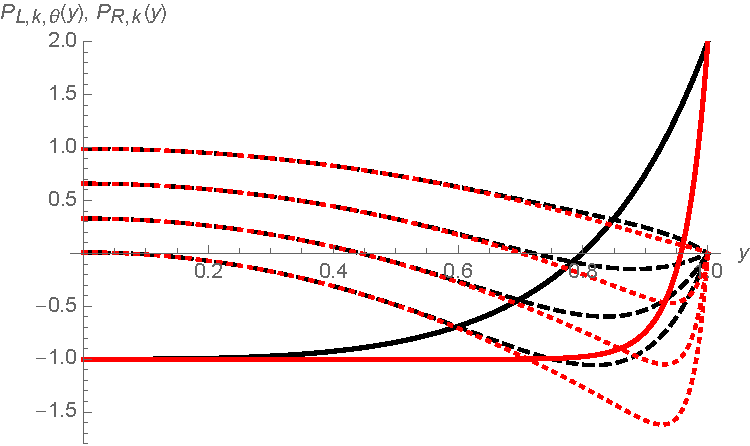
\includegraphics[width=0.5\textwidth]{fig_someplpr.pdf}
\caption{The two solid curves show the functions $y\mapsto\Por$ for some $k=k_0$ (solid black) and 
 $k=k_1$ (solid red) with $k_0<k_1$.  The dashed black curves show the functions $y\mapsto\Pol$ for $k=k_0$ and for various values of $\te\in(0,1]$. Finally, the dotted red curves show the functions $y\mapsto\Pol$ for $k=k_1$ and for the same values of $\te\in(0,1]$.}\label{fig_someplpr}
\end{center}
\end{figure}




In order to return to the original variables $(\te,\nu)$ from the variable $y$---based on \eqref{fromytonu},  \eqref{yrdef} and \eqref{yldef}---we define
\begin{equation}\label{nurdef}
\nur:=\frac{2\yr}{1-\yr^2}\cdot \frac{1}{\te},
\end{equation}
and similarly,
\begin{equation}\label{nuldef}
\nul:=\begin{cases}
 \frac{2\yl}{1-\yl^2}\cdot \frac{1}{\te} & \text{for } 0<\te<\frac{2k}{2k+1}\\
 +\infty & \text{for } \frac{2k}{2k+1}\le \te\le 1.
\end{cases}
\end{equation}
The value $+\infty$ is introduced here for convenience so as to make our descriptions shorter.

A reformulation of Corollary \ref{cor3} in terms of the variables $(\te,\nu)$ is given below.
\begin{corollary}\label{cor4}
For any $k\in\nplus$ and $\te\in(0,1]$ we have 
\[
M_{1,1}(2k+1,\te,\nu)\ge 0 \quad \Longleftrightarrow \quad \nu\le\nul,
\] 
and
\[
M_{1,j}(2k+1,\te,\nu)\ge 0 \text{  for each } 2\le j\le 2k+1 \quad \Longleftrightarrow \quad \nu\ge\nur.
\] 
In particular, 
\[
M_{1,j}(2k+1,\te,\nu)\ge 0 \text{  for each } 1\le j\le 2k+1  \quad \Longleftrightarrow \quad \nur\le\nu\le\nul.
\] 
\end{corollary}
\begin{proof} By taking into account Corollary \ref{cor3}, Lemmas \ref{lem3} and \ref{lem4}, and the fact that the map in \eqref{fromytonu} 
\begin{equation}\label{cor4bijection}
(0,1)\ni y\mapsto\frac{2y}{1-y^2}\in(0,+\infty)\text{ is a strictly increasing bijection,}
\end{equation}
we get for fixed $k$ and $\te$ that $\Por\ge 0$ is equivalent to $\nu\ge\nur$, and
$\Pol\ge 0$ is equivalent to $\nu\le\nul$. In particular, due to the definition of $\nul$ in \eqref{nuldef}, this last inequality means that there is no upper bound on $\nu$ for $\frac{2k}{2k+1}\le \te\le 1$.
\end{proof}
Some growth rates, monotonicity and limit properties of $\nur$ and $\nul$---defined in \eqref{nurdef}-- \eqref{nuldef}---are collected below; 
see also Figures \ref{fig_variousk} and \ref{fig_boundary}.
\begin{corollary}\label{cor5} (i) For any $k\in\nplus$ and $\te\in(0,1]$, we have $\nur<\nu_R(k+1,\theta)$, and
\begin{equation}\label{cor5lowerupper}
\frac{2 \left(\sqrt{2}+1\right)^{\frac{1}{2 k-1}}}{\left(\sqrt{2}+1\right)^{\frac{2}{2
   k-1}}-1}\cdot\frac{1}{\te}<\nur<\frac{2 \left(\sqrt{2}-1\right)^{\frac{1}{2 k+1}}}{1-\left(\sqrt{2}-1\right)^{\frac{2}{2
   k+1}}}\cdot\frac{1}{\te}.
\end{equation}
The asymptotic series for these lower and upper bounds have the form
\[
\left( \frac{2}{\ln \left(\sqrt{2}+1\right)}k\mp\frac{1}{\ln \left(\sqrt{2}+1\right)}+ {\cal{O}}\left(\frac{1}{k}\right)\right)\cdot\frac{1}{\te},
\]
being approximately
$
\left( 2.26919 k\mp1.13459+ {\cal{O}}\left(\frac{1}{k}\right)\right)\cdot\frac{1}{\te}.
$
In particular, $\lim_{k\to+\infty} \nur=+\infty$.\\
(ii) For fixed $0<\te<\frac{2k}{2k+1}$, $\nul>\nu_L(k+1,\theta)$ (and $\nul =+\infty$ for $\frac{2k}{2k+1}\le\te\le 1$). Finally, for fixed $\te\in(0,1]$, we have the limit
\begin{equation}\label{cor5klim}
\lim_{k\to+\infty} \nul=\frac{1}{1-\theta }\sqrt{\frac{2-\theta }{\theta }},
\end{equation}
and, for fixed $k\in\nplus$, the one-sided limits  
\begin{equation}\label{cor5thetalim}
\lim_{\te\to 0+0} \nul=+\infty=\lim_{\te\to\frac{2k}{2k+1}-0} \nul.
\end{equation}
\end{corollary}
\begin{proof} (\textit{i}) The monotonicity of $\nur$ in $k$ for fixed $\te$ follows from the monotonicity of 
$\yr$ in Lemma \ref{lem3} together \eqref{cor4bijection}, and inequality \eqref{cor5lowerupper} is 
just \eqref{yrasympt} under the transformation \eqref{cor4bijection}.\\
(\textit{ii}) We similarly obtain the monotonicity of $\nul$ in $k$ for fixed $\te$, and the limit \eqref{cor5klim} from Lemma \ref{lem4} via \eqref{cor4bijection}, by also noting that
%\begin{equation}\label{cor5roots}
\[
\frac{2\sqrt{\frac{\te}{2-\te}}}{1-\left(\sqrt{\frac{\te}{2-\te}}\right)^2}\cdot \frac{1}{\te}=\frac{1}{1-\theta }\sqrt{\frac{2-\theta }{\theta }}.
\]
%\end{equation}
As for the $\te\to\frac{2k}{2k+1}-0$ limit in \eqref{cor5thetalim}, we know from Lemma \ref{lem4} that $\yl\to 1$ (from below), and $\lim_{y\to 1-0}\frac{2y}{1-y^2}=+\infty$, hence $\nul\to+\infty$ when $\te\to\frac{2k}{2k+1}-0$.

One needs to take care only when evaluating the $\te\to 0+0$ limit in \eqref{cor5thetalim} for fixed $k\in\nplus$,  since $\frac{2\yl}{1-\yl^2}\to 0$ and $\frac{1}{\te}\to+\infty$ in \eqref{nuldef} when $\te\to0+0$. But 
the monotonicity of $\nul$ in $k$ for fixed $\te$, and \eqref{cor5klim} imply for any $k$ and $\te\in(0,1]$ that 
\[
\nul\ge\frac{1}{1-\theta }\sqrt{\frac{2-\theta }{\theta }},
\]
and the right-hand side tends to $+\infty$ as $\te\to 0+0$.
\end{proof}

\begin{figure}
\begin{center}
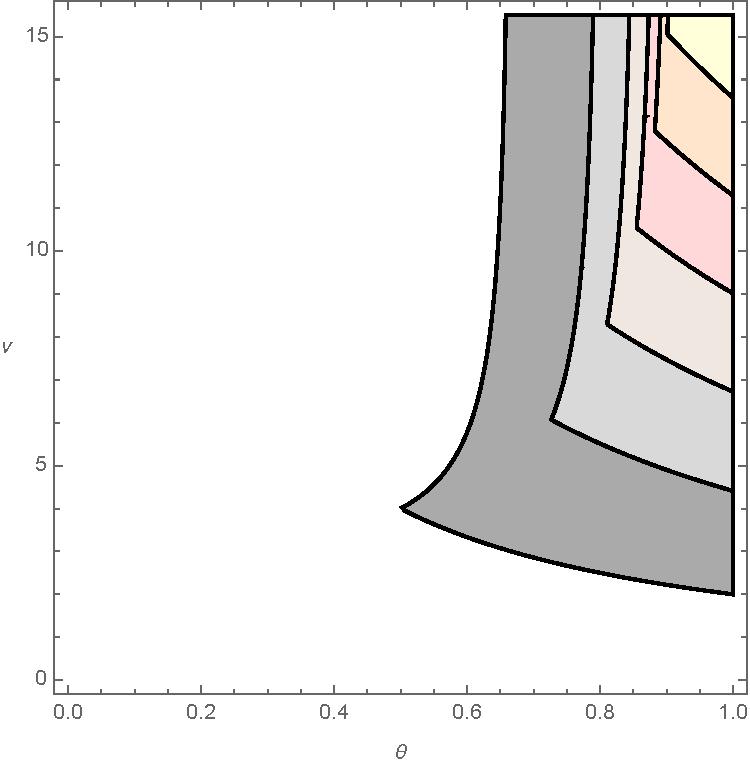
\includegraphics[width=0.48\textwidth]{fig_variousk.pdf}
\caption{The parameter regions in the $(\te,\nu)$ parameter plane ensuring $M(2k+1,\te,\nu)\ge 0$ for $k=1, 2, \ldots, 6$ (different values of $k$ are represented by different colors). The regions continue to extend to infinity ``upward'', but ``shrink'' in the horizontal direction as $k$ is increased.}\label{fig_variousk}
\end{center}
\end{figure}



\begin{figure}
\begin{center}
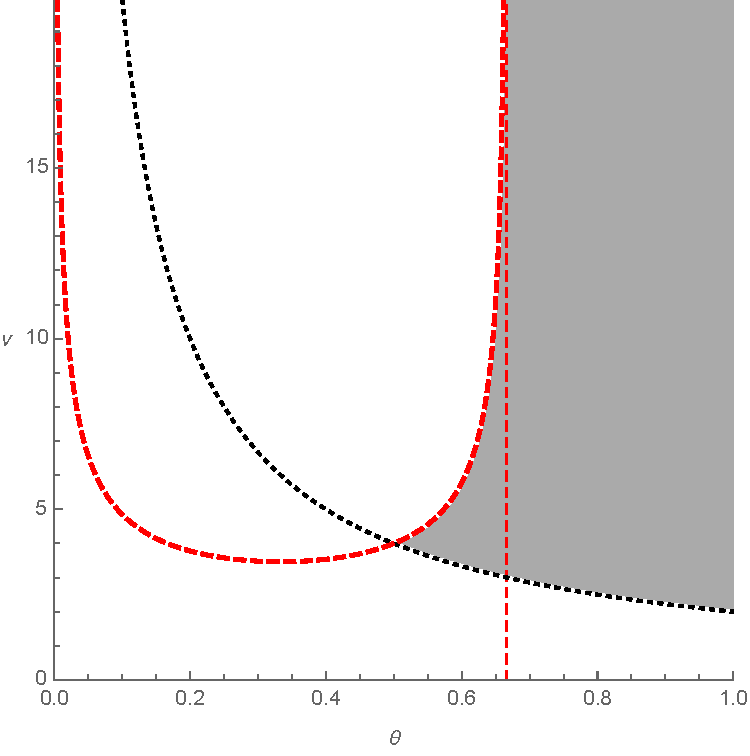
\includegraphics[width=0.48\textwidth]{fig_boundary.pdf}
\caption{A typical shaded region in Figure \ref{fig_variousk} for which $M(2k+1,\te,\nu)\ge 0$; in this particular case, for $k=1$. The gray region is described by the inequalities $\nur\le\nu\le\nul$. The black dotted curve represents the function $\te\mapsto\nur$, while the red dashed curve is the function 
$\te\mapsto\nul$, having a vertical asymptote at $\te=2k/(2k+1)$.}\label{fig_boundary}
\end{center}
\end{figure}



The following result explains why the ``left half'' of Figure \ref{fig_variousk} is ``empty'' (cf.~Corollary \ref{cor4})---the result is non-trivial, since for fixed $k$, $\lim_{\te\to 0+0} \nul=+\infty=\lim_{\te\to 0+0} \nur$ (cf.~Figure \ref{fig_boundary}).
\begin{lemma}\label{lem5} For any $k\in\nplus$ there is a unique $\te_k\in[\frac{1}{2},1)$  such that 
\[
\nur = \nul\quad \Longleftrightarrow \quad \te= \te_k.
\]
This $\te_k$ also satisfies
\[
\nur < \nul\quad \Longleftrightarrow \quad \te> \te_k.
\]
Moreover, $\te_k$ is strictly increasing in $k$, and  $\te_1=\frac{1}{2}$. In particular, for any $k\in\nplus$ and $\te\in\left(0,\frac{1}{2}\right)$ we have 
\[
 \nur>\nul.
\] 
Finally, for $\te=\te_1=1/2$
\[
M\left(2k+1,\frac{1}{2},\nu\right)\ge 0\quad\Longleftrightarrow\quad k=1\text{ and } \nu=4.
\]
\end{lemma}
\begin{proof} For $k=1$ one explicitly computes that
\[
\nu_L(1,\theta)=\frac{2}{\sqrt{\theta  (2-3 \theta)}}\quad\text{ and }\quad\nu_R(1,\theta)=\frac{2}{\te},
\]
so $\nu_L(1,\theta)=\nu_R(1,\theta) \Longleftrightarrow \te=\te_1:=1/2$ and $\nu_L(1,\theta)>\nu_R(1,\theta) \Longleftrightarrow \te>\te_1$. INCOMPLETE
\end{proof}

\begin{remark}
Thus, the ``lower left corner point'' of each shaded region in Figure \ref{fig_variousk} corresponds to a pair 
$(\te,\nu)$  for which $\nu=\nur=\nul$. This means that here the leftmost and the rightmost entries of the first row of $M(2k+1,\te,\nu)$ simultaneously vanish. For $k=1$, this happens for $\te=\te_1=1/2$ and $\nu=4$, when
\begin{equation}\label{rem10thetahalfmatrix}
M\left(3,\frac{1}{2},4\right)=\left(
\begin{array}{ccc}
 0 & 1 & 0 \\
 0 & 0 & 1 \\
 1 & 0 & 0 \\
\end{array}
\right).
\end{equation}
\end{remark}

The following theorem summarizes the results of this section in a way which is tailored to the applications. It describes the entrywise non-negativity of the discretization matrices for fixed values of $\te$---determining the actual time-integration method, then choosing the number of spatial grid points $m=2k+1$ and the CFL number $\nu$. Recall that $\te=0$ and $\te=1$ correspond to the explicit and implicit Euler methods, respectively, and $\te=1/2$ corresponds to the only second-order method in the $\te$-family. In the theorem, we assume $k\in\nplus$, $\te\in[0,1]$ and $\nu\in(0,+\infty)$.
\begin{theorem}
\begin{itemize}\ 
\item[$\bullet$] Fix $0\le\te<1/2$ arbitrarily. Then  $M(2k+1,\te,\nu)\ge 0$ can never hold, i.e., for any $k\in\nplus$ and $\nu>0$ there is at least one strictly negative entry of the matrix $M$.
\item[$\bullet$] Let $\te=1/2$. Then
\[
M\left(2k+1,\frac{1}{2},\nu\right)\ge 0\quad\Longleftrightarrow\quad k=1\text{ and } \nu=4,
\]
see \eqref{rem10thetahalfmatrix}.
\item[$\bullet$] Fix $1/2<\te<1$ arbitrarily. Then there are finitely many values of $k$ for which there exists $\nu>0$ with $M(2k+1,\te,\nu)\ge 0$. For any such value of $k$, the set of admissible values of $\nu$ has the form $\nur\le\nu\le\nul$, with suitable constants $0<\nur\le\nul\le+\infty$ (the possible case $\nul=+\infty$ means that there is no upper but only a lower bound on $\nu$); see also Corollary \ref{cor5}.
\item[$\bullet$] Let $\te=1$. Then for each $k\in\nplus$ there is a constant $\nu_R(k,1)>0$ such that
\[
M(2k+1,1,\nu)\ge 0\quad\Longleftrightarrow\quad \nu\ge\nu_R(k,1).
\]
In addition, $\nu_R(k,1)<\nu_R(k+1,1)$ for any $k$, $\lim_{k\to+\infty} \nu_R(k,1)=+\infty$, and the two-sided estimates in \eqref{cor5lowerupper} with $\te=1$ hold.
\end{itemize}
\end{theorem}
\begin{proof} The case $\te=0$ has been discussed at the beginning of Section \ref{explsect}.
In general, for $\te\in\left(0,1\right]$, we know from Corollary \ref{cor4} that for any $k$ the set of $\nu$ values for which $M(2k+1,\te,\nu)\ge 0$ holds has the form $\nur\le\nu\le\nul$. Lemma \ref{lem5} covers the range $\te\in\left(0,\frac{1}{2}\right]$. For $\te\in\left(\frac{1}{2},1\right]$ INCOMPLETE

\end{proof}






\subsection{Structured non-negative inverse eigenvalue problems}

INCOMPLETE Due to the fact that the eigenvalues of the matrix $M$ in \eqref{Mdef} are known, we can use some necessary conditions... Perron--Frobenius theorem, $\lambda_1$ non-negative real dominant root. 
It turns out that these general theorem restrict the parameter values. We give the following example.

Let us consider the $\te=1$ case. ...
These  can obtain (some weaker, why?) information on the para size of the entries $M_{i,j}$.

\section{Other discretizations}

\end{document}
